%==================================================================
%==================================================================
\section{Network embedding}
\frame{\frametitle{Outline} \tableofcontents[currentsection]}
%==================================================================
\frame{\frametitle{Network embedding: Multivariate analysis}

  \paragraph{Analysing multiple networks.} Principle
  \begin{itemize}
   \item 'Embed' each network into a convenient space (e.g. $\Rbb^d$)
   \item Use standard multivariate analysis (clustering, PCA, MDS, ...)
  \end{itemize}
  
  \bigskip \bigskip \pause
  \paragraph{Using motifs.} $K$ networks 
  $$
  (\text{Network})_k \quad \rightarrow \quad
  (N^k_1, \dots, N^k_S) \in \Rbb^S
  $$
  but need to correct for: network sizes, correlation between motif frequencies, etc...

  \bigskip \bigskip \pause
  \hspace{-.05\textwidth}
  \begin{tabular}{ll}
    \begin{tabular}{p{.4\textwidth}}
      \paragraph{~Zackenberg dataset.} $K = 46$ networks 
      \begin{itemize}
      \item 2 years
      \item 1 network observed every few days 
      \end{itemize}
    \end{tabular}
    &
    \begin{tabular}{p{.5\textwidth}}
      \includegraphics[width=.1\textwidth]{\fignet/Zackenberg-red-96:5-adj}
      \includegraphics[width=.1\textwidth]{\fignet/Zackenberg-red-96:10-adj}
      \includegraphics[width=.1\textwidth]{\fignet/Zackenberg-red-96:15-adj} 
      \includegraphics[width=.1\textwidth]{\fignet/Zackenberg-red-96:20-adj} 
      \dots \\
      \includegraphics[width=.1\textwidth]{\fignet/Zackenberg-red-97:5-adj}
      \includegraphics[width=.1\textwidth]{\fignet/Zackenberg-red-97:10-adj}
      \includegraphics[width=.1\textwidth]{\fignet/Zackenberg-red-97:15-adj} 
      \includegraphics[width=.1\textwidth]{\fignet/Zackenberg-red-97:20-adj} 
      \dots
    \end{tabular} 
  \end{tabular}

}

%==================================================================
\frame{\frametitle{Choleski transform}

  \bigskip
  \paragraph{Aim:} 'Remove' correlation and variance heterogeneity
  
  \bigskip
  \begin{tabular}{cc}
    \hspace{-0.04\textwidth}
    \begin{tabular}{p{.45\textwidth}}
      \paragraph{Covariance matrix of $(X_1, X_2)$:}
      $$
      \Sigma_{X_1, X_2} = \left[\begin{array}{cc} 
                      \sigma^2_1 & \sigma_{12} \\
                      \sigma_{12} & \sigma^2_2 \\
                     \end{array}\right]
      $$
    \end{tabular}
    & 
    \begin{tabular}{p{.45\textwidth}}
      \onslide+<2->{\paragraph{Choleski transform:}
      $$
      \left[\begin{array}{c} X'_1 \\ X'_2 \end{array} \right]
      = \Sigma^{-1/2} \left[\begin{array}{c} X_1 \\ X_2 \end{array} \right]
      $$}
    \end{tabular} 
    \\
    \hspace{-0.04\textwidth}
    \begin{tabular}{c}
      \vspace{-0.08\textheight}
      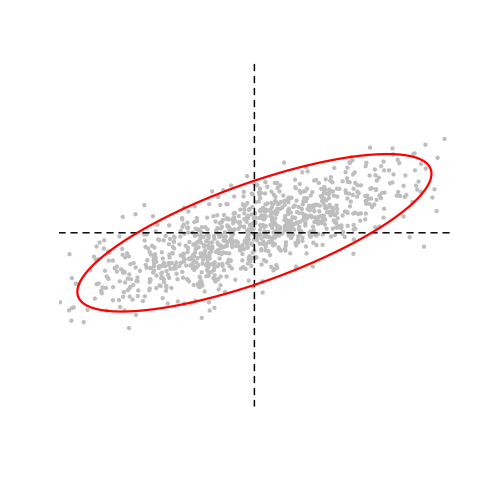
\includegraphics[width=0.35\textwidth, trim=25 25 25 25, clip=]{\fignet/Cholevski-raw} 
    \end{tabular}
    & 
    \begin{tabular}{c}
      \vspace{-0.08\textheight}
      \onslide+<2->{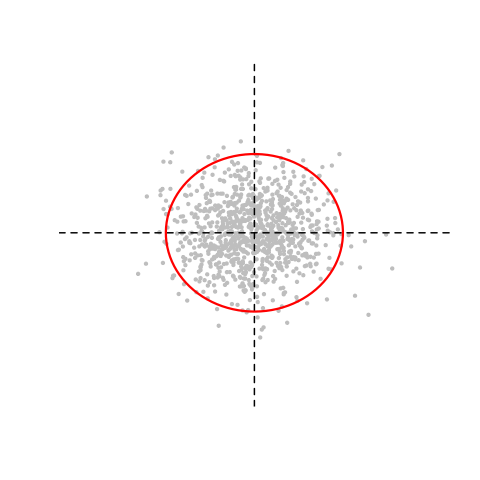
\includegraphics[width=0.35\textwidth, trim=25 25 25 25, clip=]{\fignet/Cholevski-chol}}
    \end{tabular} 
    \\
    \hspace{-0.04\textwidth}
    \begin{tabular}{p{.45\textwidth}}
      Diagonalization: $\Sigma = P \emphase{\Lambda} P^{-1}$ \\
      ~ \\
      Choleski matrix: $\Sigma^{-1/2} = P \emphase{\Lambda^{-1/2}} P^{-1}$
    \end{tabular}
    & \pause
    \begin{tabular}{p{.45\textwidth}}
      \onslide+<2->{$$
      \Sigma_{X'_1, X'_2} = \left[\begin{array}{cc} 
                      1 & 0 \\
                      0 & 1 \\
                     \end{array}\right]
      $$}
    \end{tabular} 
  \end{tabular}

}

%==================================================================
\frame{\frametitle{Network embedding: Zackenberg's data \refer{SRO16}}

  \bigskip
  \begin{tabular}{c|c|c|c}
    \onslide+<1->{Raw counts} & 
    \onslide+<2->{Corrected stat.} & 
    \onslide+<3->{Choleski} & 
    \onslide+<4>{Bray-Curtis MDS} \\
    \hline
    \onslide+<1->{\includegraphics[width=.2\textwidth, height=.175\textheight]{\fignet/Zackenberg-red-PCAcount-scree}} &
    \onslide+<2->{\includegraphics[width=.2\textwidth, height=.175\textheight]{\fignet/Zackenberg-red-PCAstat-scree}} & 
    \onslide+<3->{\includegraphics[width=.2\textwidth, height=.175\textheight]{\fignet/Zackenberg-red-PCAchol-scree}} &  
    \onslide+<4>{\includegraphics[width=.2\textwidth, height=.175\textheight]{\fignet/Zackenberg-red-MDSBrayCurtis-scree}}
    \\
    \onslide+<1->{\includegraphics[width=.22\textwidth]{\fignet/Zackenberg-red-PCAcount-biplot}} &
    \onslide+<2->{\includegraphics[width=.22\textwidth]{\fignet/Zackenberg-red-PCAstat-biplot}} &
    \onslide+<3->{\includegraphics[width=.22\textwidth]{\fignet/Zackenberg-red-PCAchol-biplot}} &
    \onslide+<4>{\includegraphics[width=.22\textwidth]{\fignet/Zackenberg-red-MDSBrayCurtis-biplot}}
    \\
    \onslide+<1->{\includegraphics[width=.2\textwidth]{\fignet/Zackenberg-red-PCAcount-size}} &
    \onslide+<2->{\includegraphics[width=.2\textwidth]{\fignet/Zackenberg-red-PCAstat-size}} &
    \onslide+<3->{\includegraphics[width=.2\textwidth]{\fignet/Zackenberg-red-PCAchol-size}} &
    \onslide+<4>{\includegraphics[width=.2\textwidth]{\fignet/Zackenberg-red-MDSBrayCurtis-size}}
  \end{tabular}

}

